\documentclass[a4paper, oneside, 12pt]{article}

% Paquets pour le Français
\usepackage[utf8]{inputenc} % Gestion encodages
\usepackage[T1]{fontenc} % ???
\usepackage[francais]{babel} % Typographie française

\usepackage{graphicx}
\usepackage{here}

\usepackage[top=2.5cm, bottom=2.5cm, left=2.5cm, right=2.5cm, footskip=.5cm]{geometry}

\newcommand\sectionSpeciale[1]{\addcontentsline{toc}{section}{#1}\section*{#1}}

\def\www{\emph{W3+}}
\def\siemens{\emph{Siemens}}

\author{ Lucien \sc{Guimier} (F5, \siemens) \\ Timothée \sc{Hamon} (F3, \www) }
\title{Dossier management}

\begin{document}

\maketitle
\thispagestyle{empty}

\newpage
\setcounter{page}{1}
\sectionSpeciale{Introduction}

\vfill

\tableofcontents

\vfill

\newpage
\section{Organisation des entreprises}

% TODO organigramme(s).
% TODO texte additionel…

\newpage
\section{Organisation des équipes}

\subsection{Organisation du travail}

À \www, le travail était organisée selon la méthodologie \emph{Scrum} : les différents projets étaient découpés en tâches courtes (une à huit heures) réparties sur une période de deux à quatre semaines. À la fin d’une telle période, le produit était en principe déployé chez le client. Chaque matin, l’équipe se réunissait pour discuter de l’avancement des tâches et des éventuels problèmes rencontrés.

\begin{figure}[H]
	\centering
	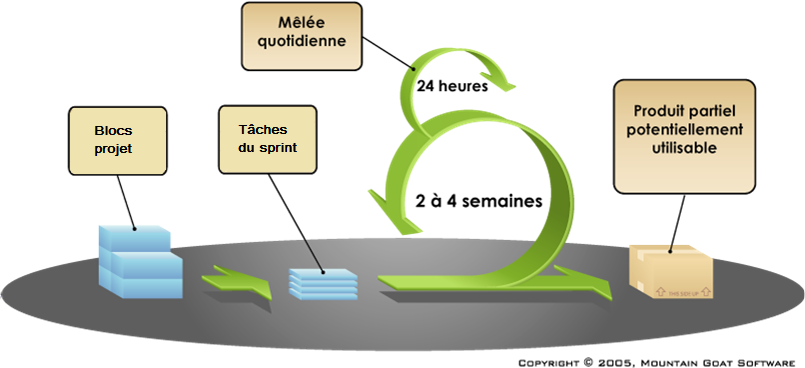
\includegraphics[width=12cm]{img/scrum.png}
	\caption{Schéma de la méthodologie \emph{Scrum}}
\end{figure}

La résolution des tâches et l’association de celle-ci avec les modifications du code étaient suivies grâce à TFS (\emph{Team Foundation Server}).

\ 

La partie de l’équipe de \siemens\ où était intégrée Lucien {\sc Guimier} se réunissait deux fois par semaine, le lundi et le mercredi, pour discuter de l’avancement des tâches. Le suivi de celles-ci était réalisé grâce à un tableau \emph{Kanban} (autre méthodologie associée à \emph{Agile}) : les tâches sont représentées par des cartons avec leur description, disposés dans des colonnes selon leur avancement (à faire, en cours, fini).

Un écran permettait d’avoir un aperçu de l’avancement de la correction des problèmes et d’être informé des prochains jalons.

\ 

Les deux méthodologies étaient assez similaires ; seule la fréquence de déploiement chez le client change : le logiciel est déployé chez \www\ au minimum une fois par mois, tandis que l’équipe de \siemens\ travaillait sur la prochaine version majeure du logiciel développé, intégrant uniquement leurs modification à la version commune, la version majeure étant publiée moins d’une fois par an.



\newpage
\section{Gestion du stagiaire}

\newpage
\sectionSpeciale{Conclusion}

\end{document}
